\chapter{\ifproject%
\ifenglish Project Structure and Methodology\else โครงสร้างและขั้นตอนการทำงาน\fi
\else%
\ifenglish Project Structure\else โครงสร้างของโครงงาน\fi
\fi
}


ในบทนี้จะกล่าวถึงหลักการ และการออกแบบระบบ

\makeatletter

% \renewcommand\section{\@startsection {section}{1}{\z@}%
%                                    {13.5ex \@plus -1ex \@minus -.2ex}%
%                                    {2.3ex \@plus.2ex}%
%                                    {\normalfont\large\bfseries}}

\makeatother
%\vspace{2ex}
% \titleformat{\section}{\normalfont\bfseries}{\thesection}{1em}{}
% \titlespacing*{\section}{0pt}{10ex}{0pt}

\section{หลักการทำงานของระบบ}

\begin{figure}[h!]
\begin{center}
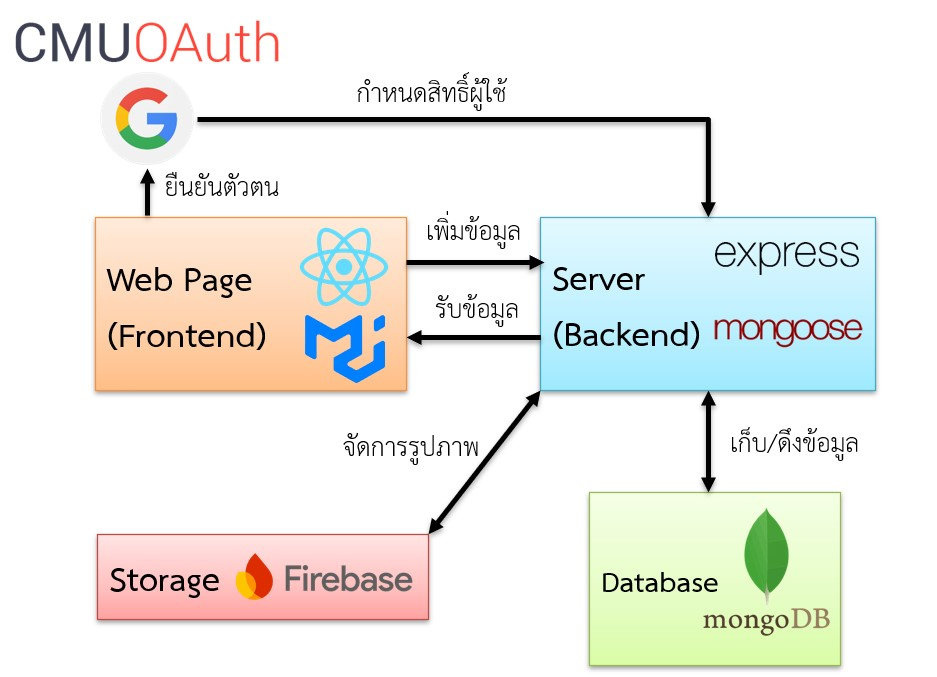
\includegraphics[scale=0.6]{public/sys-overview.jpg}
\end{center}
\caption[ภาพรวมของระบบ]{ภาพรวมของระบบ}
\label{fig:sys-overview}
\end{figure}

\subsection{ภาพรวมของระบบ}
ภาพรวมการทำงานของระบบ จะมีส่วนประกอบหลักๆ ดังนี้

\bullet{ Frontend}
ประกอบไปด้วย React Framework, โค้ด HTML, Javascript และ Material UI ใช้สำหรับแสดงผลหน้าเว็บให้แก่ผู้ใช้

\bullet{ Backend}
ประกอบไปด้วย ExpressJS, NodeJS, Mongoose และ Authorization ใช้สำหรับการทำ business logic ของระบบ

\bullet{ Database}
ประกอบไปด้วย MongoDB ใช้สำหรับเก็บข้อมูลของระบบ

\bullet{ Object Storage}
เลือกใช้บริการของ Google Firebase ในการเก็บรูปภาพกิจกรรมต่างๆ

\bullet{ Authentication}
เลือกใช้บริการ OAuth ของ Google และ CMU Account ในการเข้าสู่ระบบ
\clearpage

\subsection{โครงสร้างฐานข้อมูล}
Database ของระบบนี้ ประกอบไปด้วย 3 Collections ดังนี้

\begin{enumerate}
\item Event Collection: 
\begin{itemize}
  \item Primary Field คือ id
  \item String Fields ได้แก่ ชื่อกิจกรรม, คำอธิบายกิจกรรม, สถานที่, อีเมล, เบอร์โทรศัพท์ และ ช่องทางติดต่ออื่นๆ
  \item Array Fields ได้แก่ ประเภทกิจกรรม, คณะที่สามารถเข้าร่วมได้, path ของรูปภาพกิจกรรม และ สถานะการประกาศ
  \item Date Fields ได้แก่ วัน/เวลาเริ่มต้นกิจกรรม, วัน/เวลาสิ้นสุดกิจกรรม, วัน/เวลาประกาศกิจกรรม และ วัน/เวลาแก้ไขรายละเอียดกิจกรรม
  \item Boolean Field คือ การประกาศจากคณะ/หน่วยงาน
  \item createdBy อ้างอิงถึง Primary Field ของ User Collection (\_id)
\end{itemize}
\item User Collection:
\begin{itemize}
  \item Primary Field คือ \_id
  \item String Fields ได้แก่ ชื่อผู้ใช้, อีเมล, path ของรูป profile
  \item Array Field คือ แท็กที่ผู้ใช้สนใจ
  \item Date Fields ได้แก่ วัน/เวลาสร้างบัญชี และ วัน/เวลาแก้ไขบัญชี
  \item เนื่องจากเราใช้บริการ OAuth จึงไม่ต้องเก็บข้อมูลรหัสผ่าน
\end{itemize}
\item Review Collection: 
\begin{itemize}
  \item Primary Field คือ id
  \item user\_id อ้างอิงถึง Primary Field ของ User Collection (\_id)
  \item event\_id อ้างอิงถึง Primary Field ของ Event Collection (id)
  \item Number Field จะเก็บคะแนนในเกณฑ์ต่างๆ ได้แก่ เนื้อหา, วัน/เวลา, สถานที่ และ ทีมงาน
  \item status ใช้ระบุว่าผู้ใช้ได้กดสนใจหรือไม่
\end{itemize}
\end{enumerate}

\begin{figure}[H]
\begin{center}
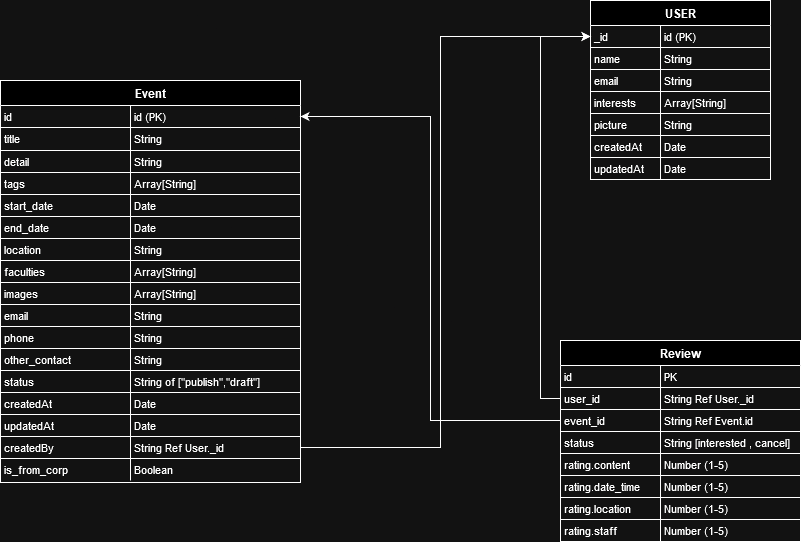
\includegraphics[scale=0.4]{public/db-diagram.png}
\end{center}
\caption[โครงสร้างฐานข้อมูล]{โครงสร้างฐานข้อมูล}
\label{fig:db-schema}
\end{figure}
\section{การใช้งานเว็บแอปพลิเคชัน}
โครงงานนี้จะแบ่งผู้ใช้ออกเป็น 2 กลุ่ม ได้แก่
\begin{enumerate}
  \item ผู้ใช้งานทั่วไป สามารถใช้งานคุณสมบัติเหล่านี้ได้ ได้แก่
  \begin{itemize}
    \item ค้นหากิจกรรม
    \item ดูรายละเอียดกิจกรรม
  \end{itemize}
  \item ผู้ใช้ที่เข้าสู่ระบบแล้ว ผ่าน Google Account หรือ CMU Account จะสามารถใช้งานคุณสมบัติได้เพิ่มขึ้น ได้แก่
  \begin{itemize}
    \item สร้างกิจกรรม
    \item กดสนใจเข้าร่วมกิจกรรม
    \item ให้คะแนนกิจกรรมที่สิ้นสุดแล้ว
    \item ดูหน้าแดชบอร์ดของเว็บ
  \end{itemize}
\end{enumerate}
\section{ส่วนเชื่อมต่อระหว่างผู้ใช้งานกับระบบ}
\subsubsection{หน้าแรก}

\begin{figure}[H]
\begin{center}
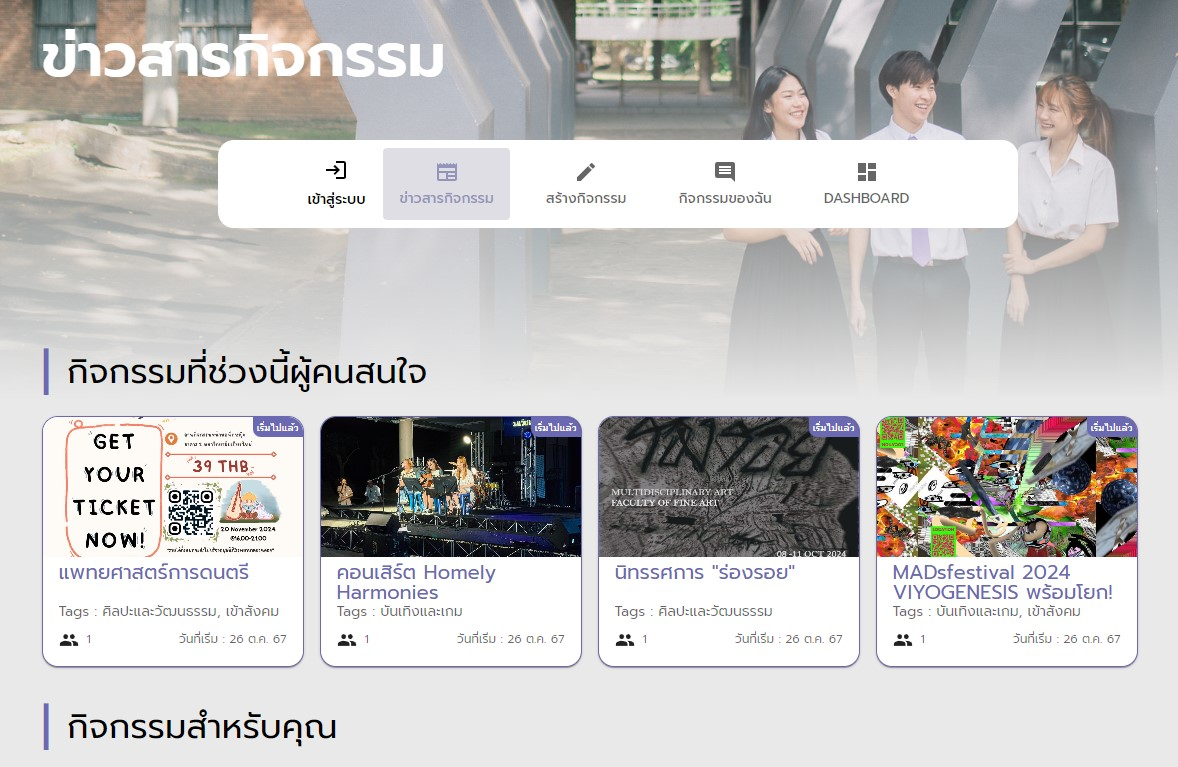
\includegraphics[scale=0.5]{public/landing.jpg}
\end{center}
\caption[หน้าแรก]{หน้าแรก}
\label{fig:landing-page}
\end{figure}
\subsubsection{หน้าเข้าสู่ระบบ}
เมื่อกดปุ่มเข้าสู่ระบบในหน้าแรก จะเปลี่ยนมาเป็นหน้านี้
\begin{figure}[H]
\begin{center}
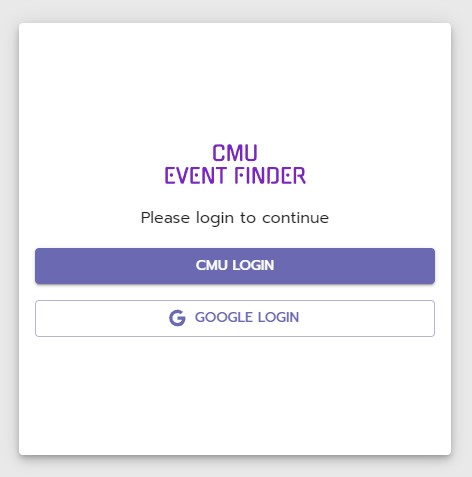
\includegraphics[scale=0.6]{public/login-page.jpg}
\end{center}
\caption[หน้าเข้าสู่ระบบ]{หน้าเข้าสู่ระบบ}
\label{fig:login-page}
\end{figure}
\subsubsection{หน้าเลือกประเภทกิจกรรมที่สนใจ}
เมื่อเข้าสู่ระบบครั้งแรก ผู้ใช้จะต้องเลือกประเภทกิจกรรมที่สนใจ โดยความสนใจเหล่านี้สามารถเปลี่ยนแปลงภายหลังได้
\begin{figure}[H]
\begin{center}
\fbox{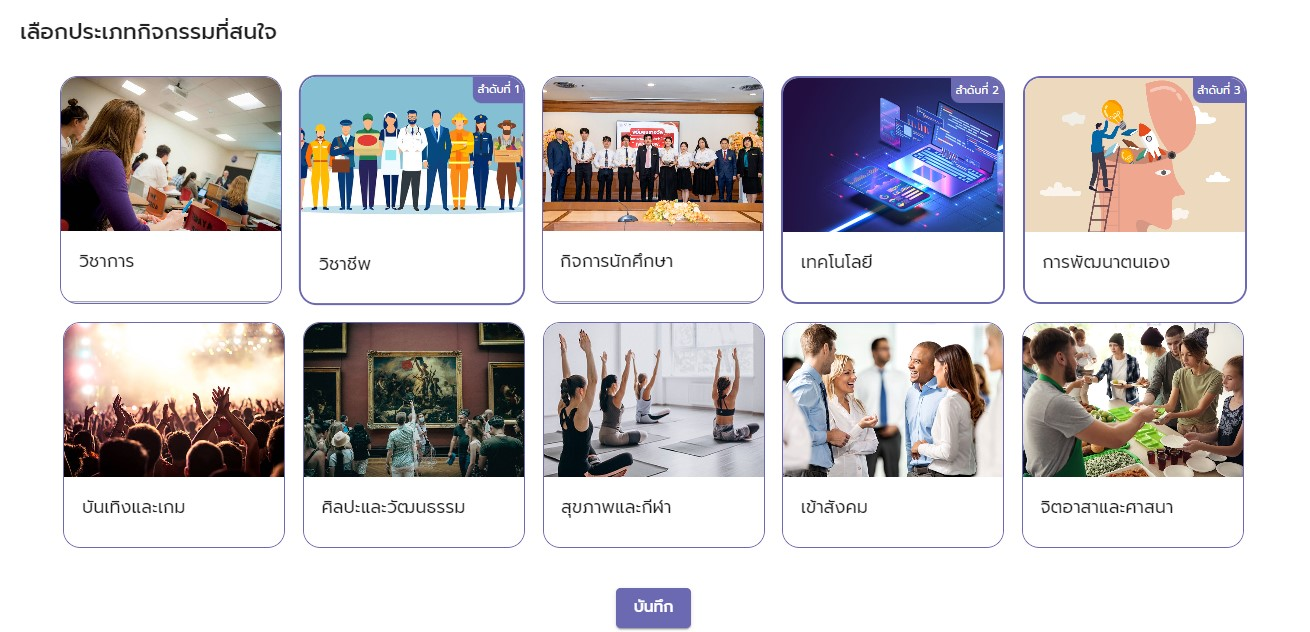
\includegraphics[scale=0.5]{public/tag-choose.jpg}}
\end{center}
\caption[หน้าเลือกประเภทกิจกรรมที่สนใจ]{หน้าเลือกประเภทกิจกรรมที่สนใจ}
\label{fig:tag-choose}
\end{figure}
\subsubsection{หน้าสร้างกิจกรรม}
\begin{figure}[H]
\begin{center}
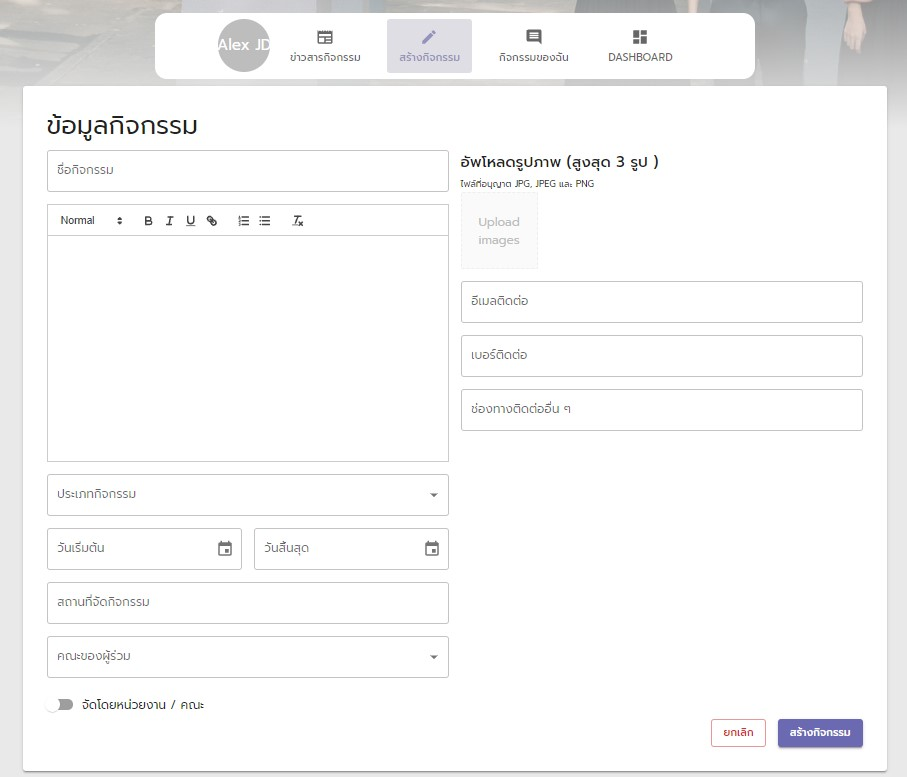
\includegraphics[scale=0.6]{public/create-act.jpg}
\end{center}
\caption[หน้าสร้างกิจกรรม]{หน้าสร้างกิจกรรม}
\label{fig:create-page}
\end{figure}
\subsubsection{หน้ากิจกรรมของฉัน}
ประกอบด้วยกิจกรรมที่สร้าง และกิจกรรมที่กดสนใจเข้าร่วม
\begin{figure}[H]
\begin{center}
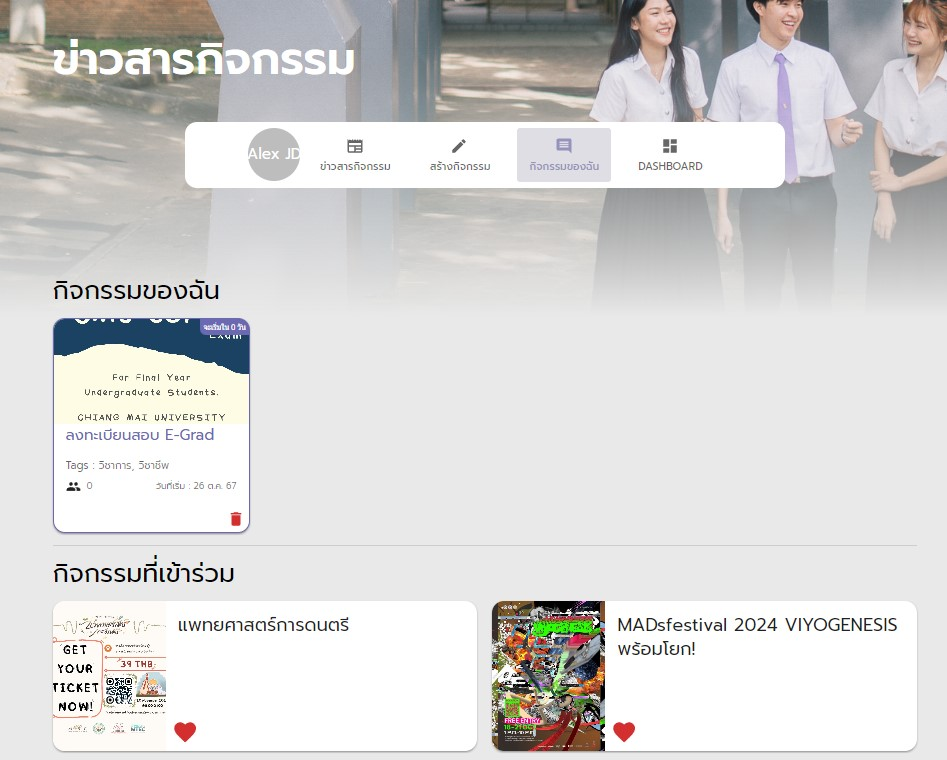
\includegraphics[scale=0.4]{public/my-act.jpg}
\end{center}
\caption[หน้ากิจกรรมของฉัน]{หน้ากิจกรรมของฉัน}
\label{fig:my-event-page}
\end{figure}
\subsubsection{หน้าแดชบอร์ด}
สามารถดูสถิติโดยรวมของเว็บได้
\begin{figure}[H]
\begin{center}
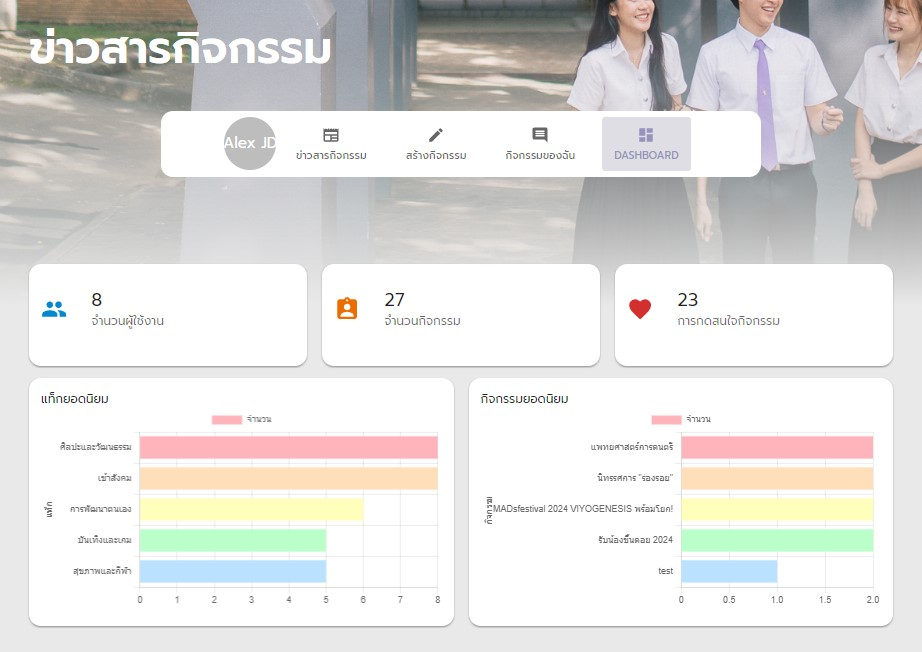
\includegraphics[scale=0.5]{public/dash-page.jpg}
\end{center}
\caption[หน้าแดชบอร์ด]{หน้าแดชบอร์ด}
\label{fig:dashboard-page}
\end{figure}
\clearpage
\subsubsection{รายละเอียดกิจกรรมโดยย่อ}
จะแสดงรายละเอียดโดยย่อของกิจกรรม
\begin{figure}[H]
\begin{center}
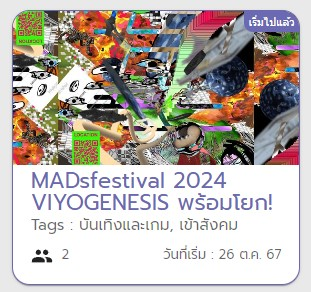
\includegraphics[scale=0.8]{public/act-mini.jpg}
\end{center}
\caption[รายละเอียดกิจกรรมโดยย่อ]{รายละเอียดกิจกรรมโดยย่อ}
\label{fig:event-box}
\end{figure}

\subsubsection{หน้ารายละเอียดทั้งหมดของกิจกรรม}
\begin{figure}[H]
\begin{center}
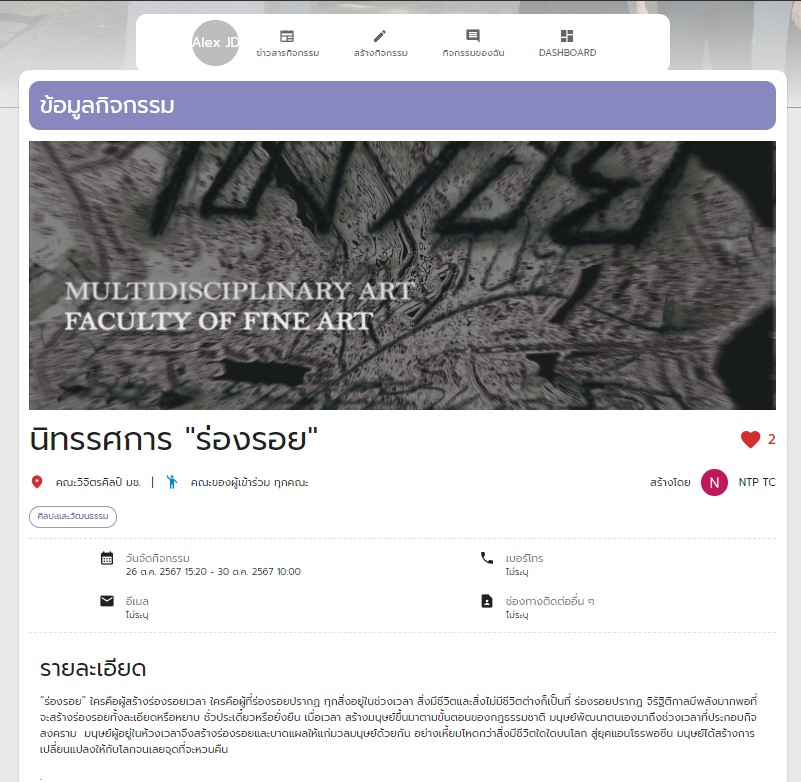
\includegraphics[scale=0.5]{public/act-detail.jpg}
\end{center}
\caption[หน้ารายละเอียดทั้งหมดของกิจกรรม]{หน้ารายละเอียดทั้งหมดของกิจกรรม}
\label{fig:event-detail}
\end{figure}
\clearpage
\subsubsection{หน้าต่างให้คะแนนกิจกรรม}
เมื่อกดปุ่ม "กรุณาให้คะแนน" หน้าต่างให้คะแนนกิจกรรมจะแสดงขึ้นมา
\begin{figure}[H]
\begin{center}
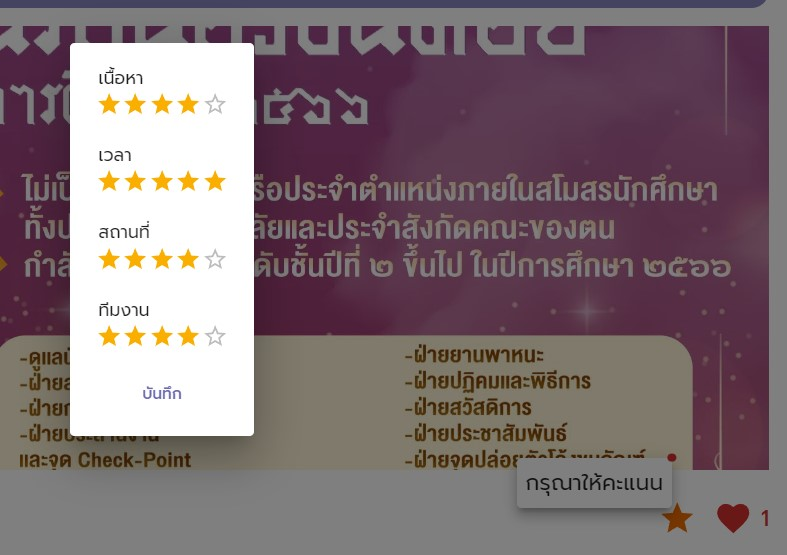
\includegraphics[scale=0.6]{public/act-review.jpg}
\end{center}
\caption[หน้าต่างให้คะแนนกิจกรรม]{หน้าต่างให้คะแนนกิจกรรม}
\label{fig:review-window}
\end{figure}
\subsubsection{ส่วนแสดงคะแนนกิจกรรม}
ในหน้ารายละเอียดกิจกรรมของกิจกรรมที่สิ้นสุดแล้ว จะแสดงคะแนนเฉลี่ยของกิจกรรม
\begin{figure}[H]
\begin{center}
\fbox{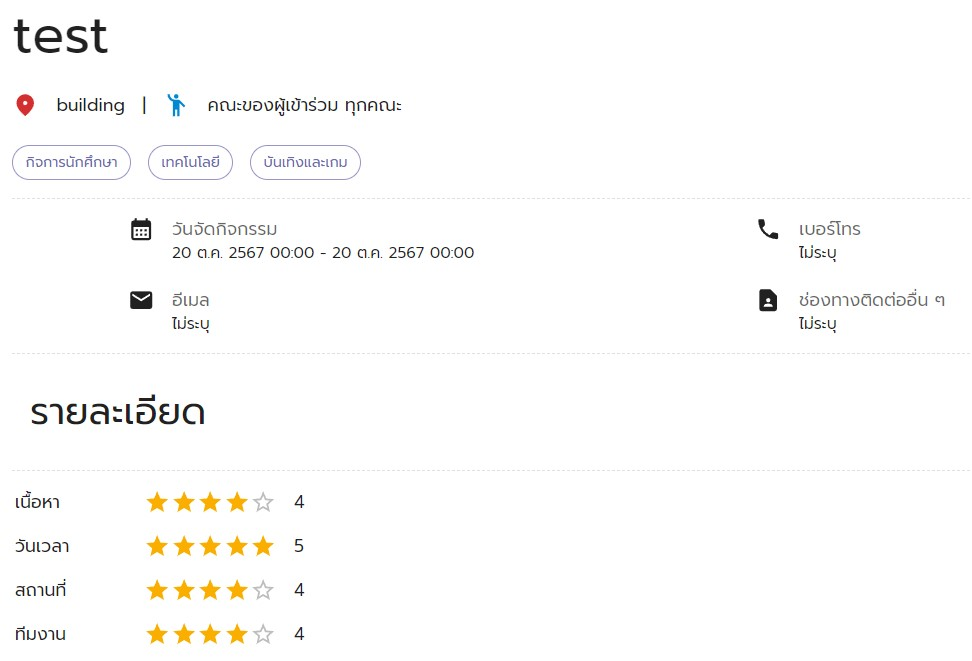
\includegraphics[scale=0.5]{public/act-score.jpg}}
\end{center}
\caption[ส่วนแสดงคะแนนกิจกรรม]{ส่วนแสดงคะแนนกิจกรรม}
\label{fig:score-section}
\end{figure}


